\PassOptionsToPackage{unicode=true}{hyperref} % options for packages loaded elsewhere
\PassOptionsToPackage{hyphens}{url}
\PassOptionsToPackage{dvipsnames,svgnames*,x11names*}{xcolor}
%
\documentclass[10pt,ignorenonframetext,]{beamer}
\usepackage{pgfpages}
\setbeamertemplate{caption}[numbered]
\setbeamertemplate{caption label separator}{: }
\setbeamercolor{caption name}{fg=normal text.fg}
\beamertemplatenavigationsymbolsempty
% Prevent slide breaks in the middle of a paragraph:
\widowpenalties 1 10000
\raggedbottom
\setbeamertemplate{part page}{
\centering
\begin{beamercolorbox}[sep=16pt,center]{part title}
  \usebeamerfont{part title}\insertpart\par
\end{beamercolorbox}
}
\setbeamertemplate{section page}{
\centering
\begin{beamercolorbox}[sep=12pt,center]{part title}
  \usebeamerfont{section title}\insertsection\par
\end{beamercolorbox}
}
\setbeamertemplate{subsection page}{
\centering
\begin{beamercolorbox}[sep=8pt,center]{part title}
  \usebeamerfont{subsection title}\insertsubsection\par
\end{beamercolorbox}
}
\AtBeginPart{
  \frame{\partpage}
}
\AtBeginSection{
  \ifbibliography
  \else
    \frame{\sectionpage}
  \fi
}
\AtBeginSubsection{
  \frame{\subsectionpage}
}
\usepackage{lmodern}
\usepackage{amssymb,amsmath}
\usepackage{ifxetex,ifluatex}
\usepackage{fixltx2e} % provides \textsubscript
\ifnum 0\ifxetex 1\fi\ifluatex 1\fi=0 % if pdftex
  \usepackage[T1]{fontenc}
  \usepackage[utf8]{inputenc}
  \usepackage{textcomp} % provides euro and other symbols
\else % if luatex or xelatex
  \usepackage{unicode-math}
  \defaultfontfeatures{Ligatures=TeX,Scale=MatchLowercase}
\fi
\usetheme[]{Singapore}
\usefonttheme{serif}
% use upquote if available, for straight quotes in verbatim environments
\IfFileExists{upquote.sty}{\usepackage{upquote}}{}
% use microtype if available
\IfFileExists{microtype.sty}{%
\usepackage[]{microtype}
\UseMicrotypeSet[protrusion]{basicmath} % disable protrusion for tt fonts
}{}
\IfFileExists{parskip.sty}{%
\usepackage{parskip}
}{% else
\setlength{\parindent}{0pt}
\setlength{\parskip}{6pt plus 2pt minus 1pt}
}
\usepackage{xcolor}
\usepackage{hyperref}
\hypersetup{
            pdftitle={Module 8: Tree-based Methods},
            pdfauthor={Stefanie Muff, Department of Mathematical Sciences, NTNU},
            colorlinks=true,
            linkcolor=Maroon,
            filecolor=Maroon,
            citecolor=Blue,
            urlcolor=blue,
            breaklinks=true}
\urlstyle{same}  % don't use monospace font for urls
\newif\ifbibliography
\usepackage{color}
\usepackage{fancyvrb}
\newcommand{\VerbBar}{|}
\newcommand{\VERB}{\Verb[commandchars=\\\{\}]}
\DefineVerbatimEnvironment{Highlighting}{Verbatim}{commandchars=\\\{\}}
% Add ',fontsize=\small' for more characters per line
\usepackage{framed}
\definecolor{shadecolor}{RGB}{248,248,248}
\newenvironment{Shaded}{\begin{snugshade}}{\end{snugshade}}
\newcommand{\AlertTok}[1]{\textcolor[rgb]{0.94,0.16,0.16}{#1}}
\newcommand{\AnnotationTok}[1]{\textcolor[rgb]{0.56,0.35,0.01}{\textbf{\textit{#1}}}}
\newcommand{\AttributeTok}[1]{\textcolor[rgb]{0.77,0.63,0.00}{#1}}
\newcommand{\BaseNTok}[1]{\textcolor[rgb]{0.00,0.00,0.81}{#1}}
\newcommand{\BuiltInTok}[1]{#1}
\newcommand{\CharTok}[1]{\textcolor[rgb]{0.31,0.60,0.02}{#1}}
\newcommand{\CommentTok}[1]{\textcolor[rgb]{0.56,0.35,0.01}{\textit{#1}}}
\newcommand{\CommentVarTok}[1]{\textcolor[rgb]{0.56,0.35,0.01}{\textbf{\textit{#1}}}}
\newcommand{\ConstantTok}[1]{\textcolor[rgb]{0.00,0.00,0.00}{#1}}
\newcommand{\ControlFlowTok}[1]{\textcolor[rgb]{0.13,0.29,0.53}{\textbf{#1}}}
\newcommand{\DataTypeTok}[1]{\textcolor[rgb]{0.13,0.29,0.53}{#1}}
\newcommand{\DecValTok}[1]{\textcolor[rgb]{0.00,0.00,0.81}{#1}}
\newcommand{\DocumentationTok}[1]{\textcolor[rgb]{0.56,0.35,0.01}{\textbf{\textit{#1}}}}
\newcommand{\ErrorTok}[1]{\textcolor[rgb]{0.64,0.00,0.00}{\textbf{#1}}}
\newcommand{\ExtensionTok}[1]{#1}
\newcommand{\FloatTok}[1]{\textcolor[rgb]{0.00,0.00,0.81}{#1}}
\newcommand{\FunctionTok}[1]{\textcolor[rgb]{0.00,0.00,0.00}{#1}}
\newcommand{\ImportTok}[1]{#1}
\newcommand{\InformationTok}[1]{\textcolor[rgb]{0.56,0.35,0.01}{\textbf{\textit{#1}}}}
\newcommand{\KeywordTok}[1]{\textcolor[rgb]{0.13,0.29,0.53}{\textbf{#1}}}
\newcommand{\NormalTok}[1]{#1}
\newcommand{\OperatorTok}[1]{\textcolor[rgb]{0.81,0.36,0.00}{\textbf{#1}}}
\newcommand{\OtherTok}[1]{\textcolor[rgb]{0.56,0.35,0.01}{#1}}
\newcommand{\PreprocessorTok}[1]{\textcolor[rgb]{0.56,0.35,0.01}{\textit{#1}}}
\newcommand{\RegionMarkerTok}[1]{#1}
\newcommand{\SpecialCharTok}[1]{\textcolor[rgb]{0.00,0.00,0.00}{#1}}
\newcommand{\SpecialStringTok}[1]{\textcolor[rgb]{0.31,0.60,0.02}{#1}}
\newcommand{\StringTok}[1]{\textcolor[rgb]{0.31,0.60,0.02}{#1}}
\newcommand{\VariableTok}[1]{\textcolor[rgb]{0.00,0.00,0.00}{#1}}
\newcommand{\VerbatimStringTok}[1]{\textcolor[rgb]{0.31,0.60,0.02}{#1}}
\newcommand{\WarningTok}[1]{\textcolor[rgb]{0.56,0.35,0.01}{\textbf{\textit{#1}}}}
\setlength{\emergencystretch}{3em}  % prevent overfull lines
\providecommand{\tightlist}{%
  \setlength{\itemsep}{0pt}\setlength{\parskip}{0pt}}
\setcounter{secnumdepth}{0}

% set default figure placement to htbp
\makeatletter
\def\fps@figure{htbp}
\makeatother

\usepackage{multirow}

\title{Module 8: Tree-based Methods}
\providecommand{\subtitle}[1]{}
\subtitle{TMA4268 Statistical Learning V2021}
\author{Stefanie Muff, Department of Mathematical Sciences, NTNU}
\date{March 8 and 9, 2021}

\begin{document}
\frame{\titlepage}

\begin{frame}{Example 2: Detection of Minor Head Injury}
\protect\hypertarget{example-2-detection-of-minor-head-injury}{}

\tiny

(Artificial data) \vspace{2mm}

\normalsize

\begin{itemize}
\item
  Data from patients that enter hospital. The aim is to quickly assess
  whether a patient as a brain injury or not (binary outcome =
  classification problem).
\item
  Patients are investigated and (possible) asked questions.
\item
  Our job: To build a good model to predict quickly if someone has a
  brain injury. The method should be

  \begin{itemize}
  \item
    \textbf{easy} to interpret for the medical personell that are not
    skilled in statistics, and
  \item
    \textbf{fast}, such that the medical personell quickly can identify
    a patient that needs treatment.
  \end{itemize}
\end{itemize}

\(\rightarrow\) This can be done by using tree-based methods.

\vspace{4mm}

\small

Note: Of course, the model should be built \emph{before} a new emergency
patient arrives, using data that is already available.

\end{frame}

\begin{frame}[fragile]

The dataset includes data about 1321 patients and is a modified and
smaller version of the (simulated) dataset \texttt{headInjury} from the
\texttt{DAAG} library.

\footnotesize

\begin{verbatim}
##    amnesia bskullf GCSdecr GCS.13 GCS.15 risk consc oskullf vomit brain.injury
## 3        0       0       0      0      0    0     0       0     0            0
## 9        0       0       0      0      0    1     0       0     0            0
## 11       0       0       0      0      0    0     0       0     0            0
## 12       1       0       0      0      0    0     0       0     0            0
## 14       0       0       0      0      0    0     0       0     0            0
## 16       0       0       0      0      0    0     0       0     0            0
##    age
## 3   44
## 9   67
## 11  62
## 12   1
## 14  55
## 16  63
\end{verbatim}

\normalsize

\end{frame}

\begin{frame}[fragile]

\begin{itemize}
\tightlist
\item
  The variable \texttt{brain.injury} will be the response of our model
  (=1 if a person has an acute brain injury, =0 otherwise).
\end{itemize}

\vspace{0mm}

\begin{itemize}
\tightlist
\item
  250 (19\%) of the patients have a clinically important brain injury.
\end{itemize}

\vspace{0mm}

\begin{itemize}
\item
  The 10 variables used as explanatory variables describe the state of
  the patient, for example

  \begin{itemize}
  \tightlist
  \item
    Is he/she vomiting?
  \item
    Is the Glasgow Coma Scale (GCS)
    score\footnote{The GCS scale goes back to an article in the Lancet in 1974, and is used to describe the level of consciousness of patients with an acute brain injury. See <https://www.glasgowcomascale.org/what-is-gcs/>}
    after 2 hours equal to 15 (or not)?
  \item
    Has he/she an open scull fracture?
  \item
    Has he/she had a loss of consciousness?
  \item
    and so on.
  \end{itemize}
\end{itemize}

\end{frame}

\begin{frame}

The classification tree made from a training set of 850 randomly drawn
observations (training set) for the head injury example looks like this:

\begin{center}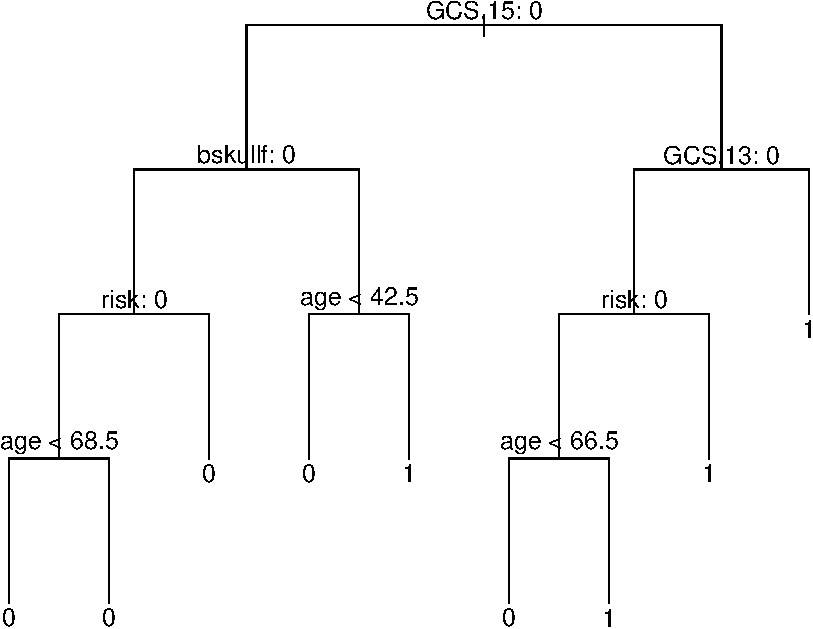
\includegraphics[width=0.7\linewidth]{Leftovers_8Trees_files/figure-beamer/injury1-1} \end{center}

\small

Note: The split criterion at each node is to the left. For example,
``GCS.15:0'' means that ``GCS.15=0'' goes left, and ``GCS.15=1'' goes
right.

\end{frame}

\begin{frame}[fragile]

\footnotesize

\begin{Shaded}
\begin{Highlighting}[]
\KeywordTok{print}\NormalTok{(headtree)}
\end{Highlighting}
\end{Shaded}

\begin{verbatim}
## node), split, n, deviance, yval, (yprob)
##       * denotes terminal node
## 
##  1) root 850 819.00 0 ( 0.8129 0.1871 )  
##    2) GCS.15: 0 711 520.00 0 ( 0.8805 0.1195 )  
##      4) bskullf: 0 663 398.00 0 ( 0.9110 0.0890 )  
##        8) risk: 0 487 203.00 0 ( 0.9466 0.0534 )  
##         16) age < 68.5 445 131.00 0 ( 0.9663 0.0337 ) *
##         17) age > 68.5 42  48.30 0 ( 0.7381 0.2619 ) *
##        9) risk: 1 176 170.00 0 ( 0.8125 0.1875 ) *
##      5) bskullf: 1 48  66.20 1 ( 0.4583 0.5417 )  
##       10) age < 42.5 13  11.20 0 ( 0.8462 0.1538 ) *
##       11) age > 42.5 35  43.60 1 ( 0.3143 0.6857 ) *
##    3) GCS.15: 1 139 192.00 1 ( 0.4676 0.5324 )  
##      6) GCS.13: 0 121 167.00 0 ( 0.5289 0.4711 )  
##       12) risk: 0 78 101.00 0 ( 0.6538 0.3462 )  
##         24) age < 66.5 66  77.30 0 ( 0.7273 0.2727 ) *
##         25) age > 66.5 12  13.50 1 ( 0.2500 0.7500 ) *
##       13) risk: 1 43  52.70 1 ( 0.3023 0.6977 ) *
##      7) GCS.13: 1 18   7.72 1 ( 0.0556 0.9444 ) *
\end{verbatim}

\normalsize

\end{frame}

\begin{frame}

\begin{itemize}
\item
  By using simple decision rules related to the most important
  explanatory variables the medical staff can now assess the probability
  of a brain injury.
\item
  The decision can go ``top down'', because the most informative
  predictors are usually split first.
\item
  Example: The staff might check if the Glasgow Coma Scale of the
  patient is 15 after 2h, and if it was 13 at the beginning. In that
  case, the probability of brain injury is estimated to be 0.944 (node 7
  in printout).
\end{itemize}

\textbf{Advantages}:

\begin{itemize}
\item
  Decision trees are easier to interpret than many of the classification
  (and regression) methods that we have studied so far.
\item
  Decision trees provide an easy way to visualize the data for
  non-statisticians.
\end{itemize}

\end{frame}

\end{document}
